%!TEX root = ZagHexaFinalReport.tex
%!TEX encoding = UTF-8 Unicode
%==============================================================================

In today’s technological society, people have grown accustomed to daily use of several kinds of technology from personal computers to supercomputers, from personal vehicles to commercial airplanes, from mobile phones to communicating through the Internet and everything in between. Robotics technology has been a hot topic recent years.  As such, the use of robots has become increasingly common. As robots can be used to complete repeated tasks, increase manufacturing production, carry extra weight and many other common tasks that humans do. Therefore, robots can be found everywhere. \\

So far, all mobile robots used in extraterrestrial surface exploration missions were wheel-driven systems. However, even if such a system is equipped with a suspension system, the capability to surmount obstacles and to conquer steep inclinations is limited. Also driving on fine-grained soil can become a problem for these kind of systems. Multi-legged walking systems, in contrast, are equipped with a highly flexible locomotor system. Along with appropriate control strategies it should offer them the capability to securely maneuver in rough and steep environments. Major counter arguments for legged systems are the higher complexity regarding the mechanical design and control as well as the comparatively high power consumption. Thus, the challenge lies in minimizing these drawbacks and in exploiting the potentialities of such systems. \\

One of the most important part of a robot is its chassis. There are several basic chassis types: wheeled, tracked and legged chassis. Wheeled chassis are fast, but not suitable for rough terrain. Tracked chassis are slower, but more suitable to rugged terrain. Legged chassis are quite slow and more difficult to control, but extremely robust in rough terrain. Legged chassis are capable to cross-large holes and can operate even after losing a leg \cite{1}. Extensive research is conducted in this field because of its large potential. Legged chassis are especially ideal for space missions \cite{2,3} . There are also several projects in military research \cite{4,5}.\\
One of the interesting features of hexapod robots such as our ZagHexa (shown in \ref{fig1}) is that they can climb over obstacles larger than the equivalent sized wheeled or trucked vehicle. In fact, the use of wheels or crawlers limits the size of the obstacle that can be climbed to half the diameter of the wheels. On the contrary, legged robots can overcome obstacles that are comparable with the size of the machine leg\cite{2}. Hexapod walking robots also benefit from a lower impact on the terrain and have greater mobility in natural surroundings. This is especially important in dangerous environments like mine fields, or where it is essential to keep the terrain largely undisturbed for scientific reasons \cite{3}.
\begin{figure}
    \centering
    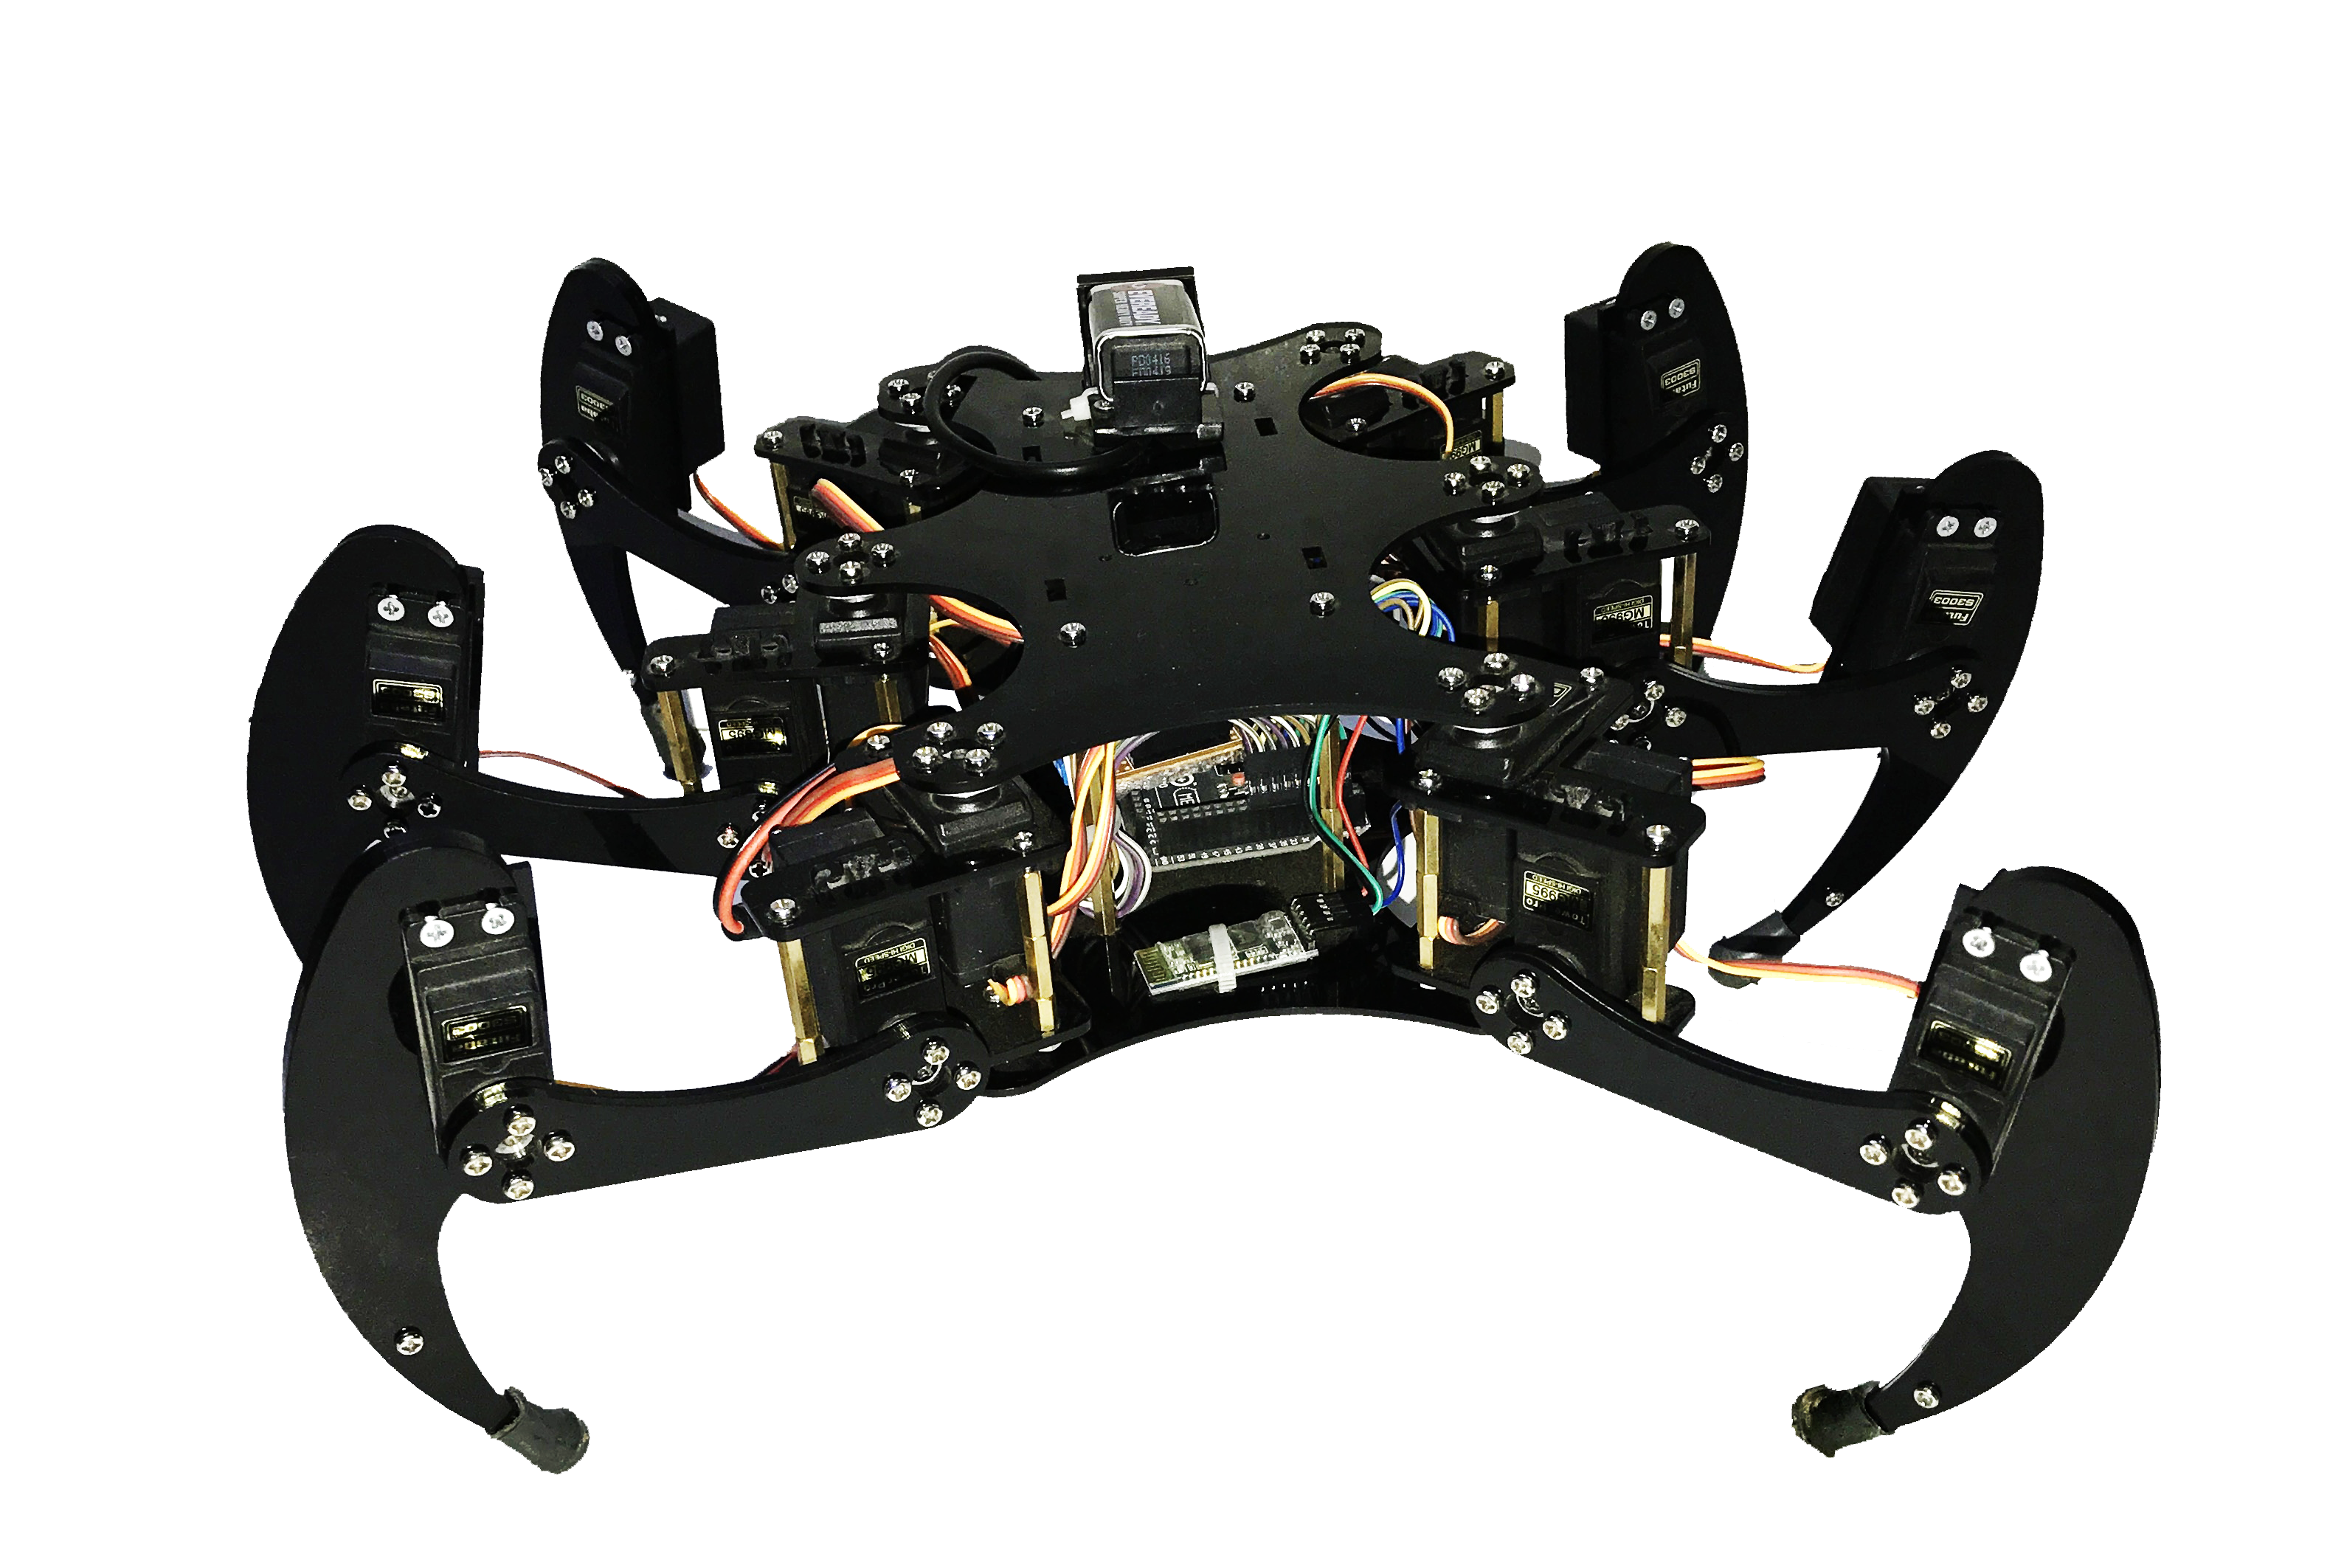
\includegraphics[width =0.9\textwidth]{ZagHexaFinal}
    \caption{ZagHexa: A sex-legged walking robot.}
    \label{fig1}
\end{figure}
Hexapod legged robots have been used in exploration of remote locations and hostile environments such as seabed \cite{4}, in space or on planets \cite{5,6}  in nuclear power stations \cite{7}, and in search and rescue operations\cite{8}. Beyond this type of application, hexapod walking vehicles can also be used in a wide variety of tasks such as forests harvesting, in aid to humans in the transport of cargo, as service robots and entertainment. Development of hexapods is increasingly robust in the military sector. Armies all over the world are exploring ways of using hexapods to detect land mines, traverse rocky, unstable terrain, and carry out simple delivery missions in danger zones.

\section{State of the Art} 
Robots inspired by insects and other animals have previously been designed with physical antennae and tactile sensors to navigate their environment, as in the work by Brooks (1989) \cite{20,22}, Cowan et al. (2005), Hartmann (2001) \cite{27} and Lee et al. (2008) \cite{10}; the last three works employed the use of a single tactile element rather than a pair \cite{13}.
Because of their extreme mobility and agile adaptability to irregular terrain, insects have long been an inspiration for the designers of mobile and legged robots \cite{11,14}. Early hexapod robots such as Genghis and later creations such as Tarry implemented insect-like mobility based on observations of insect behaviors. The inter- leg coordination system developed by Holk Cruse \cite{30,23}  has been widely implemented   in legged hexapods and its basis is in behavioral experiments that qualitatively analyzed insect walking behaviors \cite{18}.

\subsection{Early Designs}
The first hexapods can be identified as robots based on a rigidly predetermined motion so that
an adaptation to the ground was not possible. Early researches in the 1950s were focused on assigning the motion control completely by a human operator manually\cite{11h}. 
\begin{figure}[h]
    \centering
    \begin{tabular}{ l l }
        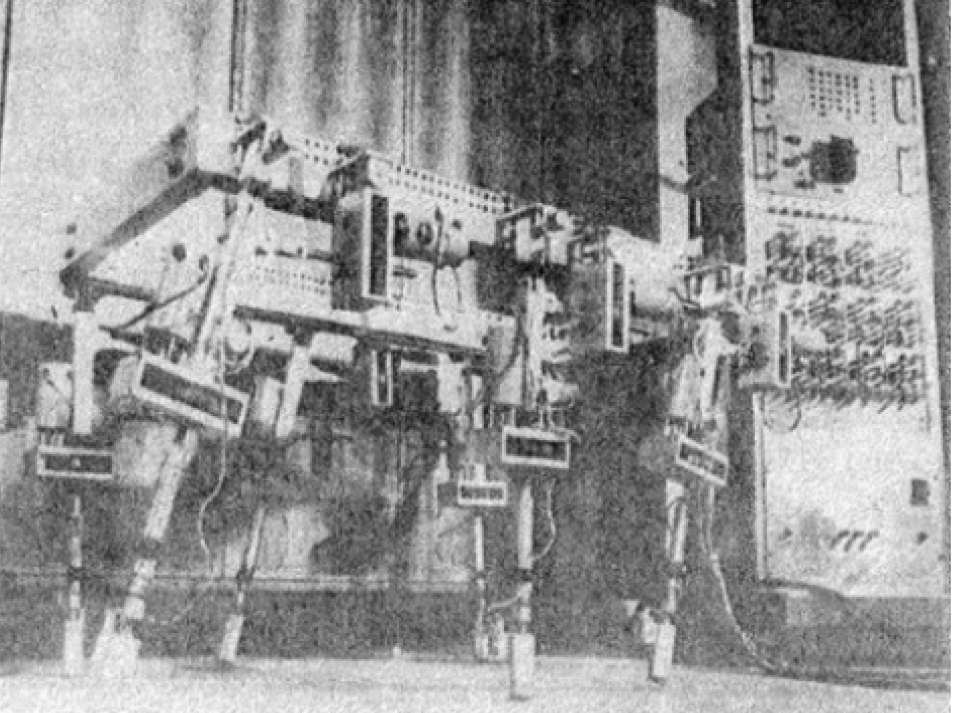
\includegraphics[width =.45\textwidth]{2_a} & 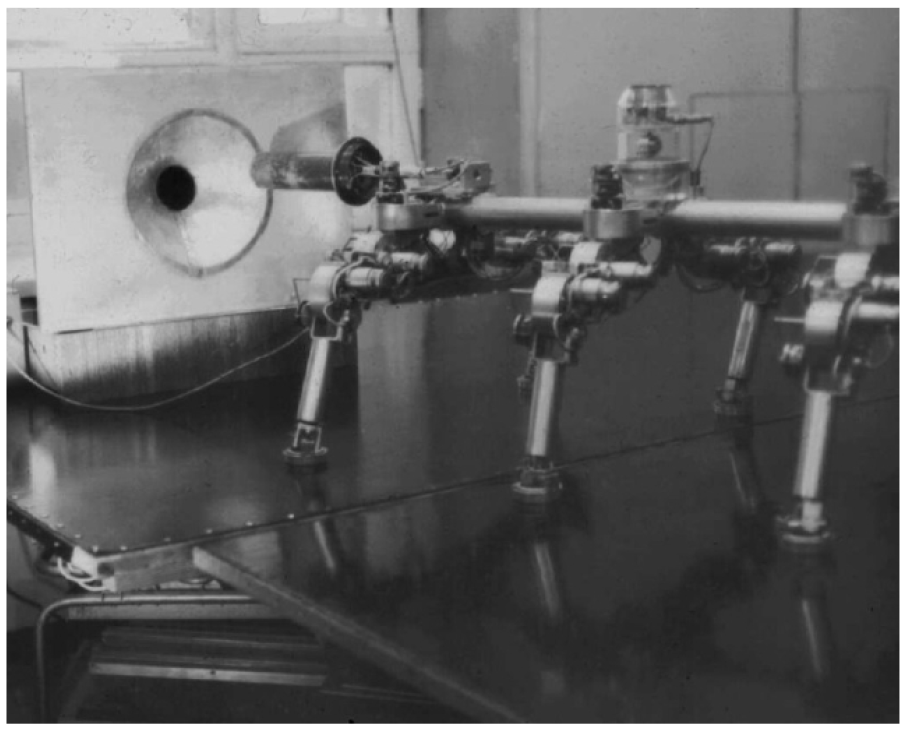
\includegraphics[width =.42\textwidth]{2_b} \\ 
        \hspace{3.5cm}(a) & \hspace{3.3cm}(b)\\
        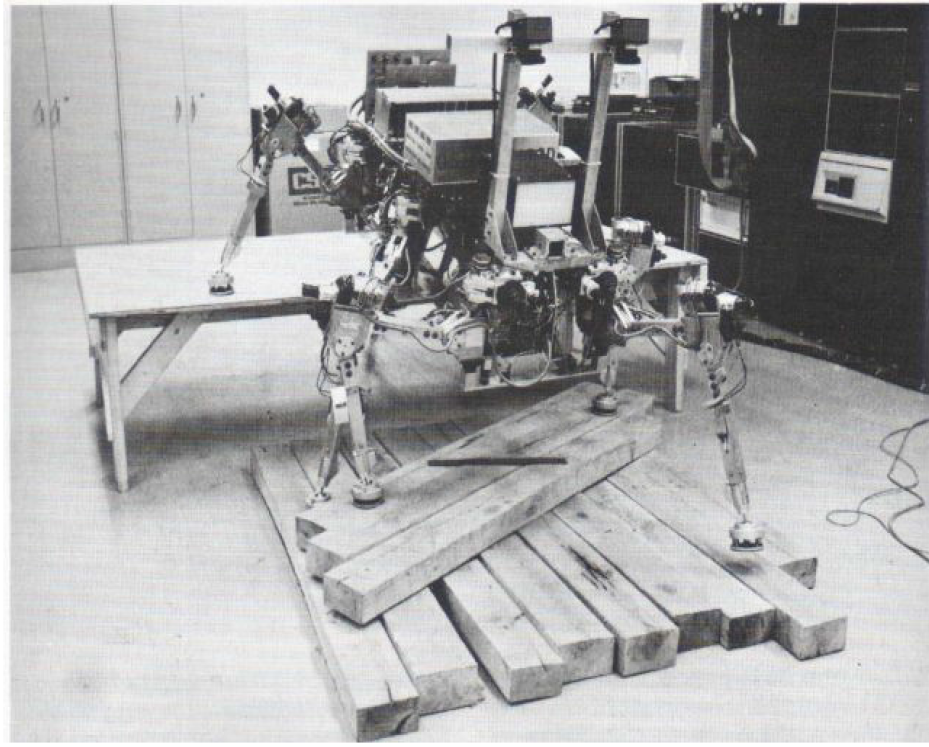
\includegraphics[width =.45\textwidth]{2_c} & \hspace{2cm} 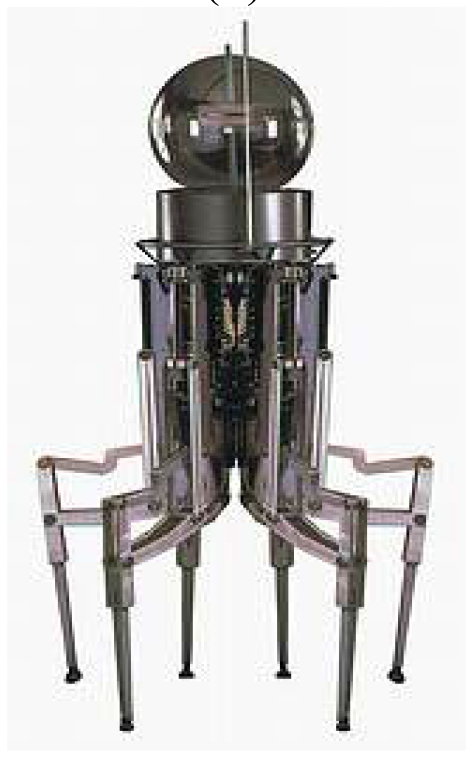
\includegraphics[width =.23\textwidth]{2_d} \\ 
        \hspace{3.5cm}(c) & \hspace{3.3cm}(d)\\
    \end{tabular}
    \caption{Early hexapod design: (a) University of Rome’s hexapod; (b) MASHA hexapod; (c) OSU hexapod; (d) ODEX I hexapod.}
    \label{fig2}
\end{figure}

One of the first successful hexapod robot was constructed at University of Rome in 1972 (\ref{fig2}a) as a computer-controlled walking machine with electric drives\cite{12h}. In the middle 70s, at the Russian Academy of Sciences in Moscow, a six-legged walking machine was developed with a mathematical model of motion control. It was equipped with a laser scanning range finder and was connected with a two-computer control system \cite{13h}. In 1976, Masha hexapod walking robot was designed at Moscow State University (\ref{fig2}b). The robot had a tubular axial chassis, articulated legs with three DoFs \cite{14h}. The hexapod was able to negotiate obstacles using contact on the feet and a proximity sensor. Ohio State University in 1977 developed a six-legged insect-like robot system called “OSU Hexapod” \cite{15h}. This hexapod was kept tethered and was made to walk short distances over obstacles (\ref{fig2}c).
In 1984, Odetic Inc., California, USA, developed Odex I \cite{17h}, a six-legged radially symmetric hexapod robot which used an onboard computer to play back pre-programmed motions (\ref{fig2}d).


\subsection{Recent Developments}
The two last decades have been characterized by a rapid development of control systems technology. Hexapod robots were equipped with various sensing systems. Artificial Intelligence systems were widely applied to the analysis of environment and motion of robots on a complex surface. A series of bio inspired robots was developed at Case Western Reserve University (USA) at the end the 90s, such as, for example, Robot III that had a total of 24 DoFs. Robot III architecture was based on the structure of cockroach, trying to imitate their behavior \cite{25h}. In particular, each rear leg had three DoFs, each middle leg four DoFs and each front leg five DoFs. Similarly, Biobot was a biomimetic robot physically modeled as the American cockroach (Periplaneta Americana) and powered by pressurized air \cite{26h}. This hexapod had a great speed and agility.

Each leg of the robot had three segments, corresponding to the three main segments of insect legs: coxa, femur, and tibia.
\begin{figure}[h]
    \centering
    \begin{tabular}{ l l }
        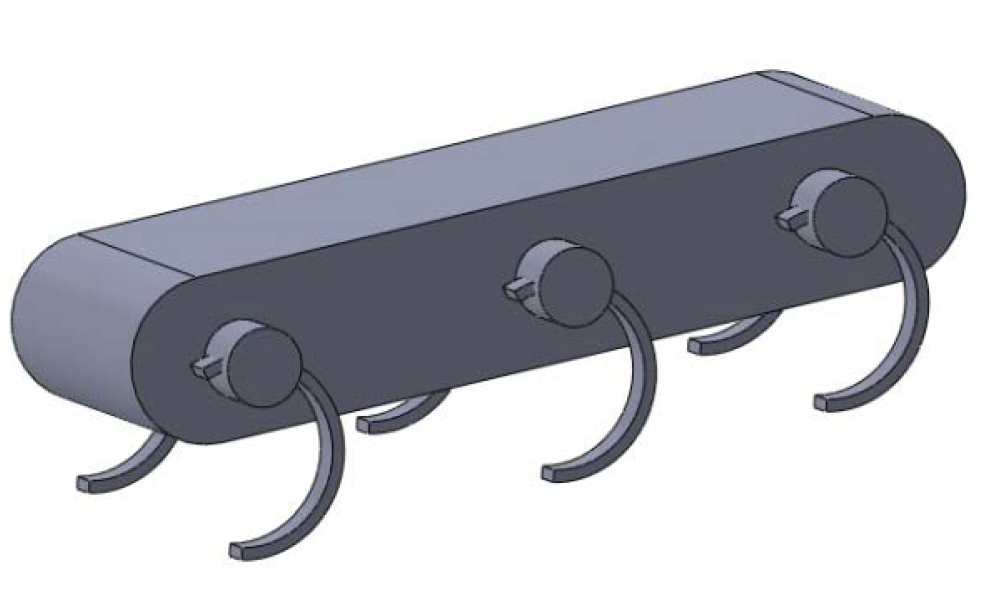
\includegraphics[width =0.45\textwidth,height=0.2\textheight]{3_a} & 
        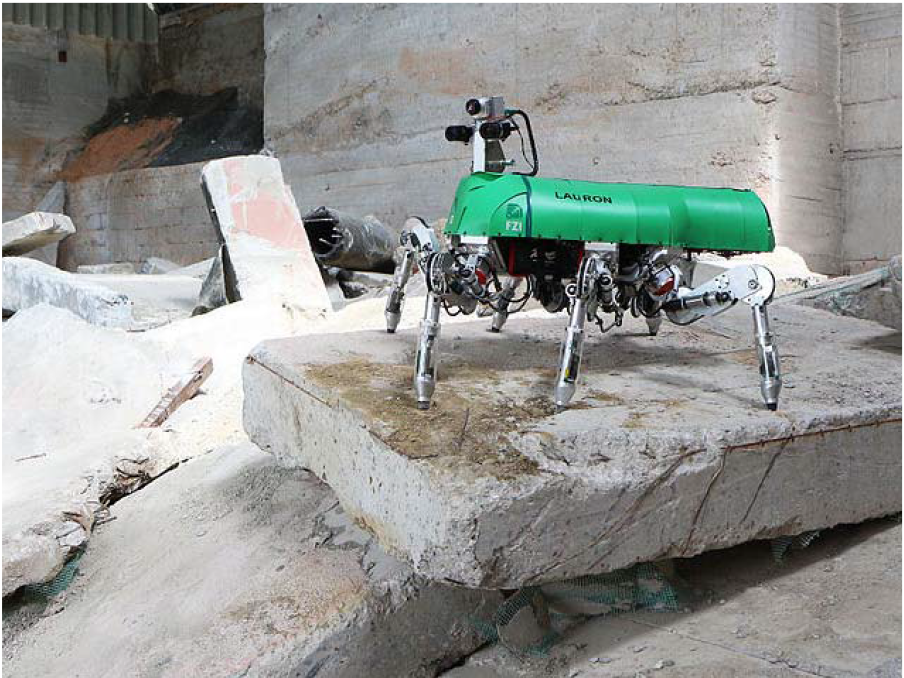
\includegraphics[width =0.45\textwidth,height=0.2\textheight]{3_b} \\ 
        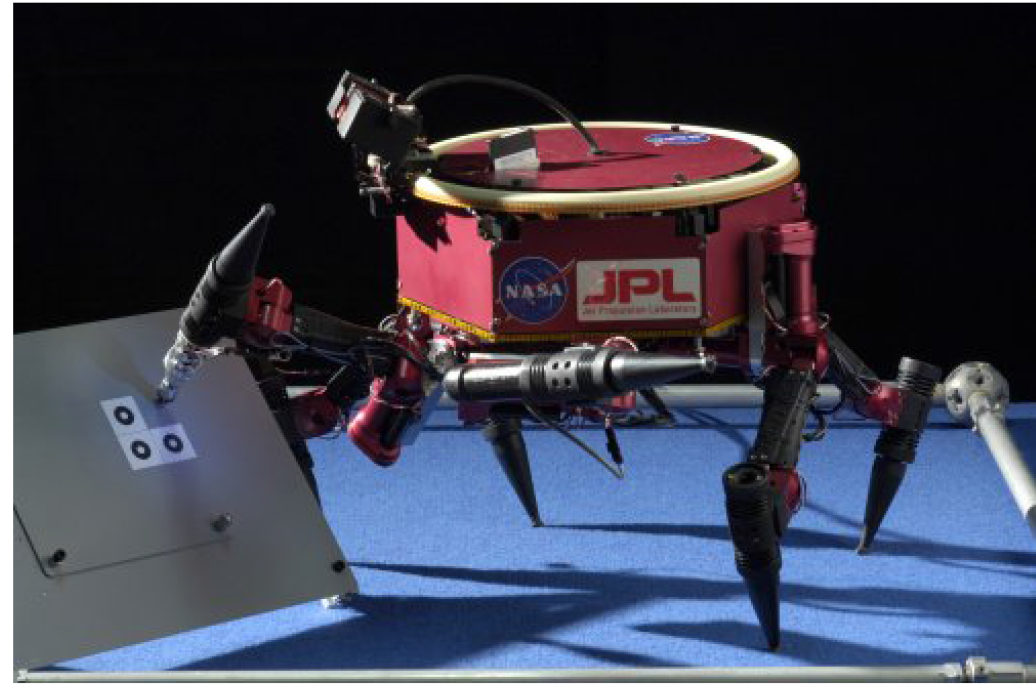
\includegraphics[width =0.45\textwidth,height=0.2\textheight]{3_c} & 
        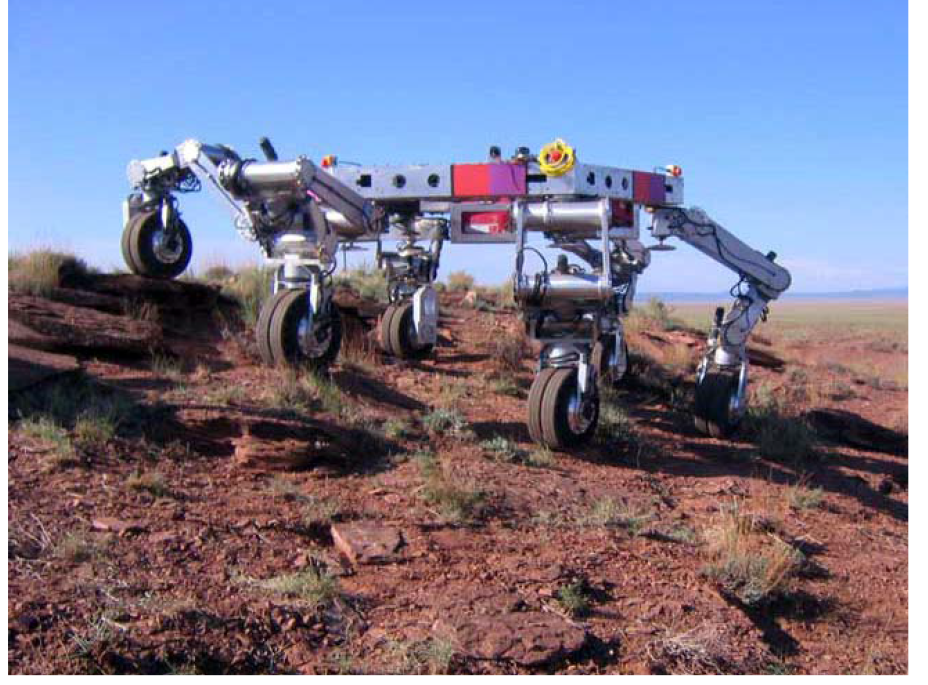
\includegraphics[width =0.45\textwidth,height=0.2\textheight]{3_d} \\ 
    \end{tabular}
    \caption{Some Example on recent developments in hexapod design}
    \label{fig3}
\end{figure}